\section{Structured Data: Pairs}
In this section, we'll introduce \textbf{structured data} to our programming language. In particular, we'll introduce \textbf{pairs}, which is essentially a two-element tuple where both elements can be anything -- numbers or pairs.

\subsection{Pair Expressions}
Our language now has the following syntax: 
\begin{verbatim}
    expr := ... | (pair <expr> <expr>) | (fst <expr>) | (snd <expr>) | nil\end{verbatim}
Here, \code{pair} defines a pair of expressions. \code{fst} and \code{snd} returns the first and second element of a pair\footnote{Although \code{fst} and \code{snd} takes any expressions, it expects a pair expression.}, respectively.

\begin{mdframed}
    (Exercise.) What will the following program evaluate to? 
    \begin{verbatim}
        (fun (inc lst)
            (if (= lst nil)
                nil
                (pair (+ (fst lst) 1) (inc (snd lst)))
            )
        )
    
    (inc (pair 70 (pair 800 nil)))\end{verbatim}

    \begin{mdframed}
        The answer is \code{(71, (801, nil))}. In this function, we first check if the given pair is \code{nil}; if it is, return \code{nil}. Otherwise, we create a new pair where the first expression is just the first element of the original pair incremented by 1, and the second element is the result of recursively calling \code{inc} on the second element of the original pair.

        \bigskip 

        We can think of the \code{(snd lst)} as the \emph{rest of the list}. 
    \end{mdframed}
\end{mdframed}

\begin{mdframed}
    (Exercise.) What will the following program evaluate to? 
    \begin{verbatim}
        (fun (sum lst)
            (let (total 0)
                (loop 
                    (if (= lst nil) 
                        (break total) 
                        (block
                            (set! total (+ total (fst lst)))
                            (set! lst (snd lst)) 
                        )
                    )
                )
            )
        )
    
        (sum (pair 70 (pair 800 nil)))\end{verbatim}
    
    \begin{mdframed}
        The answer is 870. This program iterates through each element of the pair, getting its value and adding it to \code{total}. In particular, if we ran the program, we see that 
        \begin{verbatim}        
    Expression                          (fst lst)       Total
    (pair 70 (pair 800 nil))            70              70
    (pair 800 nil)                      800             870 
    nil                                 -               -\end{verbatim}
    \end{mdframed}
\end{mdframed}

\subsection{Representing Pairs}
Recall that we used a tagging system, where we dedicated one bit, to differentiate numbers and booleans. However, with a new type, we need to rethink the tagging system. 

\bigskip 

Our tagging system will now consist of the following:
\begin{itemize}
    \item \textbf{Numbers} will still use \code{0} as its tag value.
    \item \textbf{Booleans} will use \code{11} as its tag value. 
    \begin{itemize}
        \item \code{true} will be represented in binary as \code{111} (7).
        \item \code{false} will be represented in binary as \code{011} (3).
    \end{itemize}
    \item \textbf{Pairs} will use \code{01} as its tag value. 
    \item \textbf{Nil} will use \code{1} as its tag value.
\end{itemize}
With a tagging system in hand, how do we represent pairs themselves? One approach is as follows: 
\begin{itemize}
    \item An idea is to store each of the pair's value as 31-bits. For example, to represent 2 numbers, we would represent the first number as 31 bits, and the next number as another 31 bits, with the tag value being 2 bits. 
    \item \textbf{However}, this won't really work if we have nested pairs. For example, if we have a pair with pairs as its element, then how do we represent this? 
\end{itemize}
Another thing we can think about is heap allocation. 

\subsection{Compiler Design}
As implied, we'll have to allocate pair element on the \textbf{heap} (we'll need to work with the Rust runtime for this). So, our representation is that the pair's value will be a 62-bit address on the heap. 

\bigskip 

How do we know \emph{where} to allocate pair elements on the heap? An idea is to dedicate a register that just keeps track of the current heap location. In our class, we'll use \code{r15} for our purposes. With this in mind, here are a few assumptions we will be making:
\begin{itemize}
    \item \code{r15} is expected to keep growing for now; it's not like \code{rsp} where it can increase or decrease depending on how stack space is used. 
    \item \code{r15} only refers to available memory, never used memory. 
    \item \code{r15} will be 16-byte aligned (it will end with \code{0000})
\end{itemize}
With this in mind, how do we modify our compiler to support pairs? A sketch of an implementation we'll use is as follows: 
\begin{verbatim}
    Pair(e1, e2) => {
        let fst = compile_expr(e1, ...);
        let snd = compile_expr(e2 ...);
        // e1 will be somewhere in [rsp], e2 in rax 
        format!("
            {fst}
            {snd}
            mov [r15 + 8], rax 
            mov rbx, [rsp + offset]
            mov [r15], r15
            mov rax, r15 
            add rax, 1 
            add r15, 16
        ")
    }\end{verbatim}
\textbf{Remarks:} 
\begin{itemize}
    \item We should probably first check and see if we have space left before allocating. We didn't do this part yet.  
    \item Note that we move \code{rax} into \code{[r15 + 8]} (and not \code{[r15]}) because \code{rax} has the value of the \emph{second} element of the pair, not the first. 
    \item \code{mov rax, r15} and \code{add rax, 1} is designed to put the location in heap of the pair's values into \code{rax} and then add 1 to \code{rax} for tagging purposes. Note that we can add \code{1} to \code{rax} like this because we know that \code{r15} will end with \code{0000} (this is one of the assumptions we made). 
    \item \code{add r15, 16} moves \code{r15} by 2 words, thus ensuring that it's always pointing to free memory in the heap. 
\end{itemize}
As one might have suspected, once we execute a pair, it should return the memory location to that pair. 

\subsection{Heap Allocation}
We actually have two things we need to do here: 
\begin{itemize}
    \item We need to create some sort of a \emph{heap} that our compiler can use to store pair values. Once we create 
    \item We need to put the heap pointer into \code{r15}.
\end{itemize}
Let's think about some ideas for how we can set the heap up.
\begin{itemize}
    \item One idea is to set \code{r15} to \verb|rsp - {a lot}|. In other words, if we move \code{rsp} very high up, then we can use \code{r15} as the ``heap'' pointer. \textbf{However}, let's think about the process layout:
    \begin{center}
        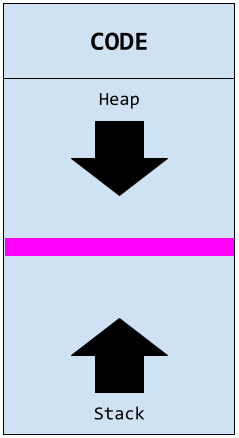
\includegraphics[scale=0.4]{assets/process_layout.png}
    \end{center}
    The typical convention is that the heap grows downwards and the stack grows upwards. In around the middle of memory (denoted by the pink rectangle), there's some special addresses where touching them will result in an error (heap overflows and stack overflows). So, if we set \code{rsp} high enough, then we might either hit that special address, or if we have a depth-heavy recursion\footnote{Since this can hit our proposed ``heap'' space.}, or if we somehow point \code{r15} to the heap space\footnote{Since this is where Rust might allocate memory, so we might end up overwriting memory that Rust needs.}, then we'll be in trouble. 

    \item We can also call Rust's equivalent of \code{malloc}, and use its value\footnote{\code{malloc} gives us the address to some allocated memory in the heap.}. In particular, 
    \begin{itemize}
        \item Call \code{malloc} for each pair\footnote{Note that heap size is \emph{unknowable} iin general \textbf{statically}.}, or 
        \item One \emph{big} \code{malloc}.
    \end{itemize}
    The suggestion we'll use is similar to having a \textbf{big} \code{malloc}. This has the added benefit of being easy to \code{free} at the end. 
\end{itemize}

\subsection{Modifying Our Rust Code}
Now, we need to modify our Rust code to account for these changes. 

\subsubsection{Modifying the Runtime}
In \code{runtime.rs}, we'll essentially do the following:
\begin{verbatim}
    fn main() {
        let args = ...;
        let input = parse_arg(&args);
        let mut memory = Vec::with_capacity(100_000);       // New!
        let buffer: *mut u64 = memory.as_mut_ptr();         // New! 
        let i: i64 = unsafe {
            our_code_starts_here(input, buffer); 
        };

        snek_print(i);
    }\end{verbatim}
Essentially, we'll create a vector with an initial capacity of \code{100\_000} elements. This will represent our heap. Then, we can get a pointer to that vector, and then pass that pointer into our generated assembly. This means our signature for \code{our\_code\_starts\_here} will look like:
\begin{verbatim}
    extern "C" {
        #[link_name = "\x01our_code_starts_here"]
        fn our_code_starts_here(input: i64, buffer: *mut u64) -> i64;
    }\end{verbatim}

\subsubsection{The Generated Assembly}
In our generated assembly, we'll have 
\begin{verbatim}
    our_code_starts_here:
        mov r15, rsi
        ...\end{verbatim}
Here, \code{rsi} represents the \emph{second} argument\footnote{Recall the x86\_64 calling convention.}. 

\subsubsection{Printing Values}
Finally, we need to adjust the \code{snek\_print} function. In particular, our function now needs to account for the fact that it can either receive 
\begin{itemize}
    \item a number (with tag \code{0}).
    \item a boolean (with tag \code{11}).
    \item a pair (with tag \code{01}).
    \item \code{nil} (with tag \code{1}).
\end{itemize}
With this in mind, we have 
\begin{verbatim}
    fn snek_str(val: i64) -> String {
        if val == 7 { "true".to_owned()} 
        else if val == 3 { "false".to_owned() } 
        else if val % 2 == 0 { format!("{}", val >> 1) } 
        else if val == 1 { "nil".to_owned() } 
        else if val & 1 == 1 {
            let addr = (val - 1) as *const i64; 
            let fst = unsafe { *addr };
            let snd = unsafe { *addr.offset(1) };
            format!("(pair {} {})", snek_str(fst), snek_str(snd))
        } else { format!("unknown value: {val}") }
    }

    #[export_name = "\x01snek_print"]
    fn snek_print(val: i64) -> i64 {
        println!("{}", snek_str(val));
        val 
    }\end{verbatim}
Note that \code{offset} is used so we don't need to do direct pointer arithmetic\footnote{We're looking at the memory location directly next to the current memory location since pairs are contiguous.}. Note that we'll need to do some work printing parentheses and whatnot.

\subsection{Memory Representation}
Suppose we have the following program: 
\begin{verbatim}
    (pair 5 (pair 6 (pair 7 nil)))\end{verbatim}
The way we compile this is to first compile the left-most part of the pair (\code{5}), and then the right-most part of the pair (the rest of the pair, in this case). In particular,
\begin{itemize}
    \item The instructions for any nested expressions get evaluated before we move those values onto the heap for the current pair.
    \begin{mdframed}
        In this program's case, we evaluate \code{5} first, and then \code{6}, and then \code{7}. We put all of them on the stack first. \emph{Then}, we put 7 onto the heap first (while \code{6} and \code{5} wait). 
    \end{mdframed}
    
    \item The first pair that gets allocated is the innermost pair. 
\end{itemize}
If we assume left-to-right evaluation order, then \code{7} goes on the heap first. In this sense, allocation happens inside-out. In any case, in the heap, we expect the memory layout to look like
\begin{center}
    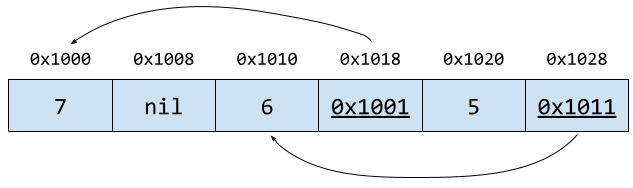
\includegraphics[scale=0.67]{assets/pair_heap.png}
\end{center}
\textbf{Remarks:} 
\begin{itemize}
    \item We have \code{0x1001} and \code{0x1011} (instead of \code{0x1000} and \code{0x1010}) because we use \code{0x01} as the tag value for the pair.
    \item Note that, in our implementation of the compiler, we're actually going to store the integer multiplied by 2 (e.g., 14, 12, and 10, respectively), since in memory we're storing the \emph{tagged} value. In this example, we're just showing the integers as is (with no tagging).
    \item This program would evaluate to \code{0x1021}, since this is the memory address to the first element in the pair. 
\end{itemize}

\begin{mdframed}
    Another way to think about this is as follows: if we wanted to translate this program into something like Python, syntactically this would look like 
    \begin{verbatim}
        p1 = (7, nil);
        p2 = (6, p1);
        p3 = (5. p2);\end{verbatim}
    We had to \emph{allocate} memory for \code{p1} (the innermost pair), and then allocate memory for \code{p2}, and then finally for \code{p3}.
\end{mdframed}

Let's now suppose we have the following program:
\begin{verbatim}
    (fun (inc lst)
        (if (= lst nil)
            nil
            (pair (+ (fst lst) 1) (inc (snd lst)))
        )
    )

    (inc (pair 70 (pair 800 nil)))\end{verbatim}
The heap diagram might look something like 
\begin{center}
    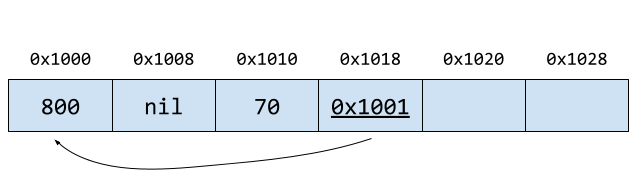
\includegraphics[scale=0.6]{assets/pair_heap2.png}
\end{center}
Here, the result of \code{(pair 70 (pair 800 nil))} is \code{0x1011}, so \code{0x1011} is passed into the \code{inc} function. If we look at the function itself, we can see that the function itself will return the same pair, pair, nil structure.
\begin{center}
    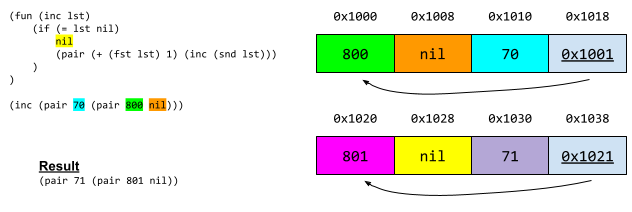
\includegraphics[scale=0.73]{assets/pair_heap3.png}
\end{center}
And, in this exmaple. this function would return \code{0x1031}, the address to the newly created pair.

\subsection{Equality}
Let's consider the following program: 
\begin{verbatim}
    (let (point1 (pair 6 5))
        (let (point2 (pair 6 5))
            (block 
                (print (= point1 point1))                       // A
                (print (= point1 point2))                       // B
                (let (pointpair1 (pair point1 point2))
                    (let (pointpair2 (pair point1 point2))
                        (block 
                            (print (= pointpair2 pointpair2))   // C
                            (print (= pointpair1 pointpair2))   // D
                        )
                    )
                )
            )
        )
    )\end{verbatim}
We now need to decide what this program should print. More specifically, however, we need to figure out how equality of pairs will work. This introduces two types of equalities:
\begin{itemize}
    \item \textbf{Reference equality:} are the two operands referring to the same memory address? For example, in Python, this is \code{==}.
    \item \textbf{Structural equality:} are the two operands equal when considering their structures? For example, in Python, this is \code{is}.
\end{itemize}
With this in mind, we have 
\begin{center}
    \begin{tabular}{|c|c|c|}
        \hline 
        Statement & Reference Equality & Structural Equality \\ 
        \hline
        A & \code{true} & \code{true} \\ 
        B & \code{false} & \code{true} \\ 
        C & \code{true} & \code{true} \\ 
        D & \code{false} & \code{true} \\ 
        \hline  
    \end{tabular}
\end{center}
Note statements (C) and (D); if we want structural equality, we probably want to do \emph{recursive structural equality!} 

\subsection{Revisiting Print}
Let's suppose we have the following program:
\begin{verbatim}
    (let (p (pair 1 2))
        (block 
            (setfst! p p)
            (print p)
        )
    )\end{verbatim}
One thing we should note is that we have a \textbf{cycle} in the sense that the pair is referring to itself. Therefore, if we tried to \code{print} the pair, we would end up with infinite recursion since we would constantly recurse through the first element of the pair. 

\bigskip 

To fix this, we should consider checking if we've \emph{seen} the pair before. If we've seen it, we can print something indicating that a cycle is detected. Otherwise, we can print out the pair as normal. 
\begin{verbatim}
    fn snek_str(val: i64, seen: &mut Vec<i64>) -> String {
        if val == 7 { "true".to_owned()} 
        else if val == 3 { "false".to_owned() } 
        else if val % 2 == 0 { format!("{}", val >> 1) } 
        else if val == 1 { "nil".to_owned() } 
        else if val & 1 == 1 {
            if seen.contains(&val) { return "...".to_owned() }
            seen.push(val);
            let addr = (val - 1) as *const i64; 
            let fst = unsafe { *addr };
            let snd = unsafe { *addr.offset(1) };
            let v = format!("(pair {} {})", snek_str(fst), snek_str(snd));
            seen.pop();
            v 
        } else { format!("unknown value: {val}") }
    }

    #[export_name = "\x01snek_print"]
    fn snek_print(val: i64) -> i64 {
        println!("{}", snek_str(val, &mut vec![]));
        val 
    }\end{verbatim}

\subsection{A Brief Sketch of Equality}
Given two pairs, how can we check if they are equal? We can use the following Rust implementation, 
\begin{verbatim}
    fn snek_eq_helper(val1: i64, val2: i64, seen: &mut Vec<(i64, i64)>) -> bool {
        if seen.contains(&(val1, val2)) { return true }

        seen.push((val1, val2));
        // continue on.
    }\end{verbatim}
The idea is that if we come across the same two cycles, we can assume that they're equal and return. Otherwise, we can evaluate the pairs as usual.